\documentclass[12pt,a4paper]{article}


\usepackage[utf8]{inputenc}
\usepackage[T1]{fontenc}
\usepackage[french]{babel}     % Typographie française
\usepackage{lmodern}           % Police vectorielle unifiée et nette
\usepackage{geometry}
\usepackage{graphicx}
\usepackage{xcolor}
\usepackage{tcolorbox}         % Pour les boites bleues
\usepackage{setspace}          % Pour l'interligne
\usepackage{titlesec}          % Pour la couleur des titres
\usepackage{hyperref}          % Pour les liens cliquables
\usepackage{amsmath}

\usepackage{pgfplotstable}
\usepackage{booktabs} % optionnel mais recommandé
\usepackage{caption}
\pgfplotsset{compat=1.18}


% Marges
\geometry{
	margin=.5cm,
	top=.5cm,
	bottom=1.2cm
}

% Interligne (1.5 pour une lecture aérée)
\onehalfspacing
\setlength{\parskip}{0.5em}

\definecolor{bleuTitre}{RGB}{0,70,140}
\definecolor{bleuCadre}{RGB}{220,235,250}

\titleformat{\section}
{\color{bleuTitre}\Large\bfseries}
{\thesection}{1em}{}

\titleformat{\subsection}
{\color{bleuTitre}\large\bfseries}
{\thesubsection}{1em}{}


\tcbset{
	colback=bleuCadre,
	colframe=bleuTitre,
	boxrule=0.8pt,
	arc=3mm,
	left=8pt, right=8pt, top=8pt, bottom=8pt
}

\begin{document}
	
	
	\begin{titlepage}
		\centering
		
		% Logo
		\begin{figure}[h]
			\centering
			% Ajustez la largeur si besoin (ex: 0.4 ou 0.6)
			
\includegraphics[width=0.5\textwidth]{logo.jpg} 
		\end{figure}
		
		\vspace{2cm}
		
		% Filet horizontal du haut
		\rule{\linewidth}{0.5mm} \\[0.4cm]
		
		% Titre
		{\color{bleuTitre} \Huge \bfseries Rapport Étude 1 - APST} \\[0.4cm]
		
		% Filet horizontal du bas
		\rule{\linewidth}{0.5mm}
		
		\vspace{1.5cm}
		
		{\Large Classification de cancer à partir de données ARN}
		
		\vfill
		
		% Bloc Informations
		\begin{minipage}{0.45\textwidth}
			\begin{flushleft} \large
				\textbf{Enseignant :} \\
				Mme \textsc{MAUMY}
			\end{flushleft}
		\end{minipage}
		\hfill
		\begin{minipage}{0.45\textwidth}
			\begin{flushright} \large
				\textbf{Étudiant :} \\
				Nathan \textsc{HASCOET}
			\end{flushright}
		\end{minipage}
		
		\vspace{2cm}
		
		% Date
		{\large \today}
		
	\end{titlepage}
	
	\section{Le jeu de données}
	
	Le jeu de donné contient 801 patients et 20 532 gênes (les variables).\\
	Dans tous les scripts fournis l'ensemble du jeux de donné a été exploité.
	
	\section{Organisation des différents scripts python}
	
	Voici une courte description des différents scripts : \\
	\hspace*{5cm}\begin{minipage}[t]{15cm}
		\begin{enumerate}
		\item[\textbf{ACP.py :}] Ce script applique bêtement une ACP sur l'ensemble du jeux de données
		
		\item[\textbf{K-means.py :}] Ce script applique un algorithme des K-means sur l'ensemble des données
		
		\item[\textbf{CAH.py :}] Ce script effectue une classification ascendante hiérarchique sur l'ensemble des données
		
		\item[\textbf{Analyse$\_$Discriminante.py :}] Analyse discriminante linéaire et quadratique sur l'ensemble des données puis sur une partie des variables synthétiques créées
	\end{enumerate}
	\end{minipage}	
		
	\begin{tcolorbox}[title=\textbf{Objectif}]
		\begin{enumerate}
			\item Être capable de prédire qu'il y a bien 5 types de cancers dans ce jeux de donnée 
			\item Réussir à prédire correctement le cancer de chacun des patients.
		\end{enumerate}
	\end{tcolorbox}	
	
	\section{ACP.py}
	
	Nous avons effectués une Analyse en composantes principales sur l'ensemble des données, n'ayant bien sûr moins de 20 532 patients, le nombre de composantes principales non nuls est inférieur ou égale à 801. Pour connaître le nombre de variable à prendre en compte pour ne pas ou perdre le moins possible d'informations, nous traçons le graphique des inerties cumulées :
	
	\begin{center}
		
\includegraphics[scale=.7]{"ACP/inertie.png"}
	\end{center}
	
	\newpage
	
	Pour obtenir $95\%$ de l'inertie totale, 530 variables (synthétiques obtenue après l'ACP) sont suffisantes. On remarque aussi que les 2 première variables ne contiennent que peux d'informations de l'inertie totales :
	
	\hspace{-1.2cm}
\includegraphics[scale=.67]{"ACP/C1_C2.png"}
\includegraphics[scale=.67]{"ACP/C2_C3.png"}
	
	Bien que l'on soit capable de réduire considérablement le nombre de variable, mais dû au fait le nombre de patients est bien moindre que le nombre de variables il semble pertinent de garder l'ensemble des variables dans un premier temps, au vu du temps de calcul nécessaire.
	
	
	\section{K-means}
	
	Aucune ACP n'a été effectué au préalable, nous avons choisi autant de classes que de cancer listés dans le jeu de donnés (5). Le nombre de fois que l'algorithme de Kmeans a été choisi à 50, et parmi ces 50 familles de centroides, la famille avec la meilleur inertie est choisie.\\
	Le taux de mal classé est assez faible malgré cela :  0.749 $\%$.
	
	\hspace{2cm}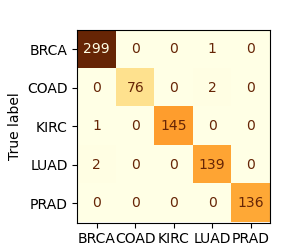
\includegraphics[scale=.7]{Kmeans/confusion_5classes.png}\hspace{3cm}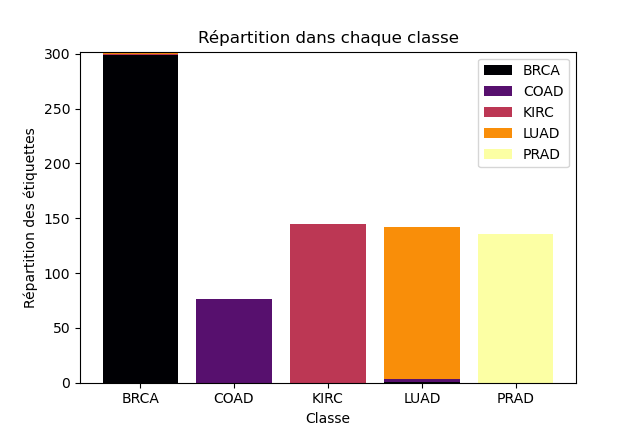
\includegraphics[scale=.4]{Kmeans/repartition_5classes.png}
	
	\hspace{-.8cm}Si l'on augmente le nombre de classe de 1 puis 2 (6 et 7 classes), et le taux de mal classé est le même pour ces 3 cas (à l'approximation choisie : 3 décimales) : 0.749 $\%$. 

	\vspace{-.33cm}
	
	\hspace{-1cm}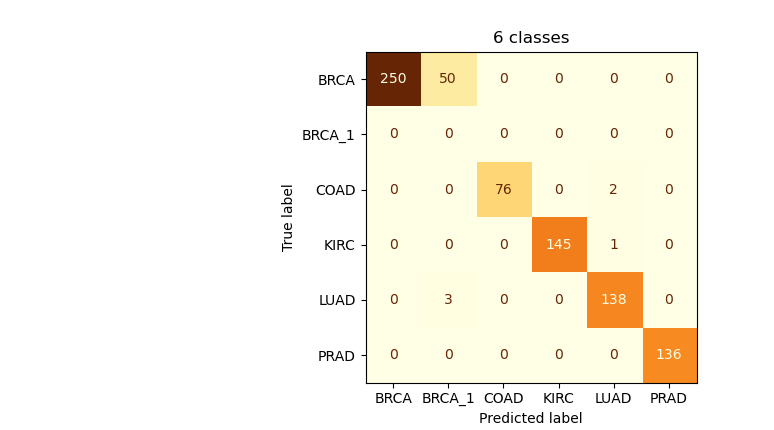
\includegraphics[scale=.5]{Kmeans/confusion_6classes.png}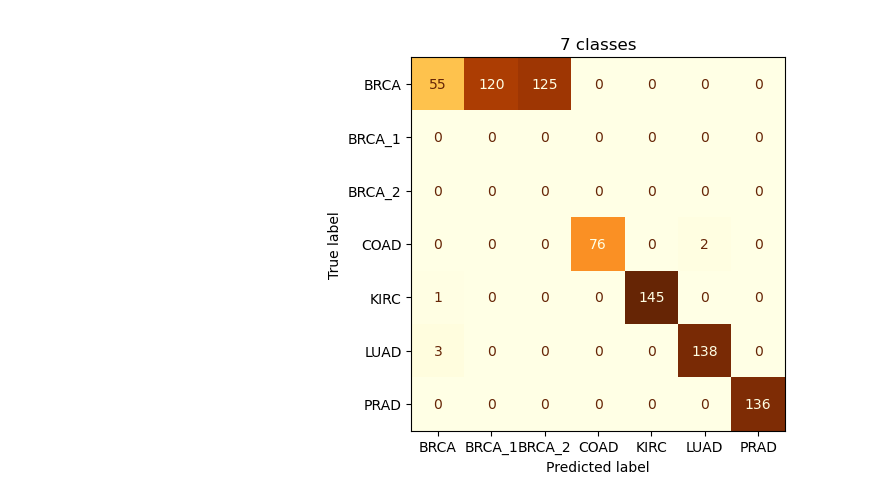
\includegraphics[scale=.45]{Kmeans/confusion_7classes.png}
	
	On remarque que dans les deux cas, la classe des cancer BRCA se scinde en 2 puis en 3, c'est un phénomène que nous allons constater aussi, d'une certaine manière, à l'aide d'une classification hiérarchique des données qui permettra de justifier ce scindage en 2 de cette catégorie.\\
	
	A partir de 3 classes en plus (donc 8 au total), le taux de mal classé diminue de  0.3 $\%$ : 0.499 $\%$\\
	Et cette fois on constate que c'est la classe de cancer nommé KIRC qui se scinde en 2.
	
	\hspace{-2cm}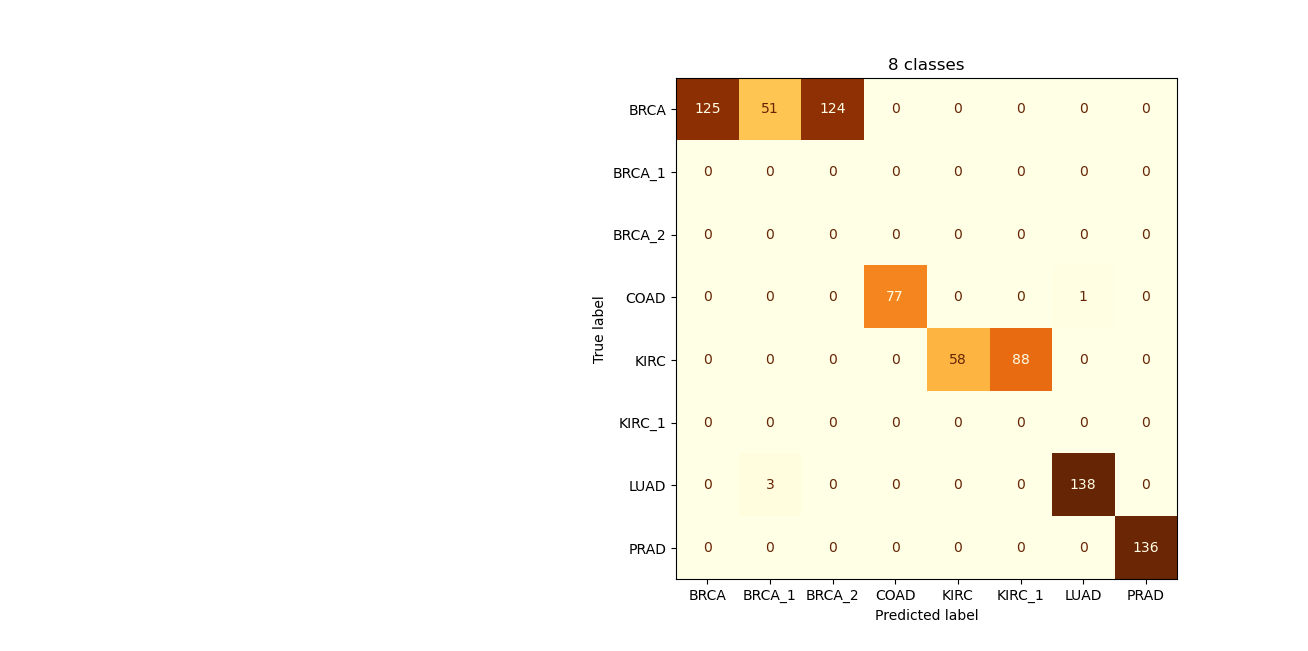
\includegraphics[scale=.5]{Kmeans/confusion_8classes.png}
	
	\vspace{-1.5cm}
	
	\section{Classification Hiérarchique Ascendante}
	
	\vspace{-.5cm}
	
	Regardons le graphique de la différence de variance interclasse lors de la fusion de 2 classes (sur l'axes des ordonnées, il a été volontairement idiqué chacune des valeurs pour visualiser les sauts) :
	
	\hspace{3.5cm}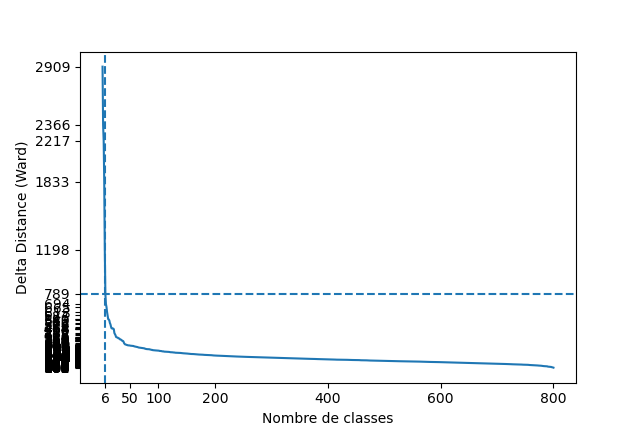
\includegraphics[scale=.6]{CAH/delta.png}
	
	On remarque qu'à partir de 789, les saut des distances sont significatifs, Changement que l'on observe sur le graphique des variance interclasse (qui correspond à la variance interclasse : 1781) : 
	
	\vspace{-.3cm}
	
	\hspace{3.5cm}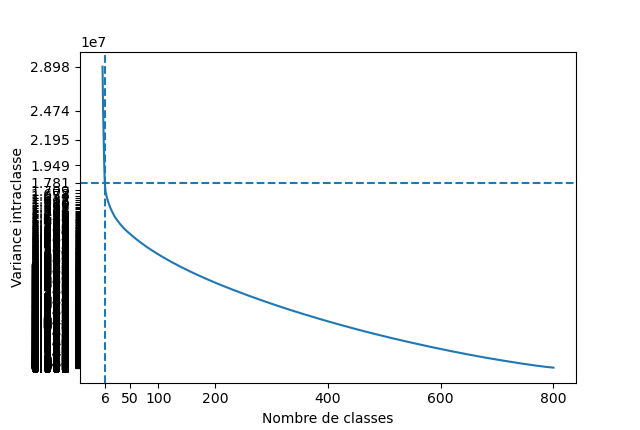
\includegraphics[scale=.5]{CAH/variance_interclasse.png}
	
	On remarque tout de suite que ce seuil (789) correspond à 6 classes et non pas 5. En choisissant ce seuil de 789 on obtient le dendrogramme suivant :
	
	\hspace*{1cm}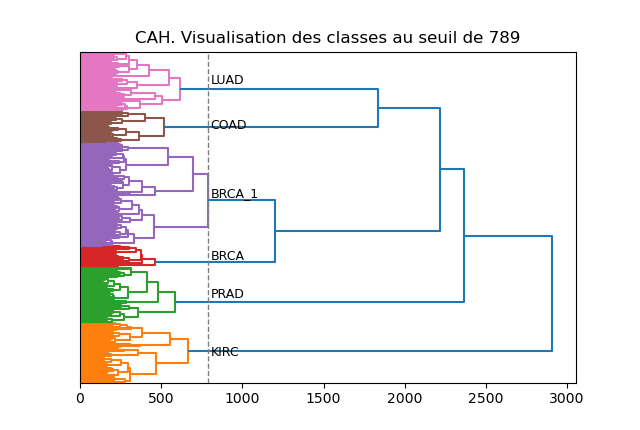
\includegraphics[scale=.5]{CAH/arbre900.png}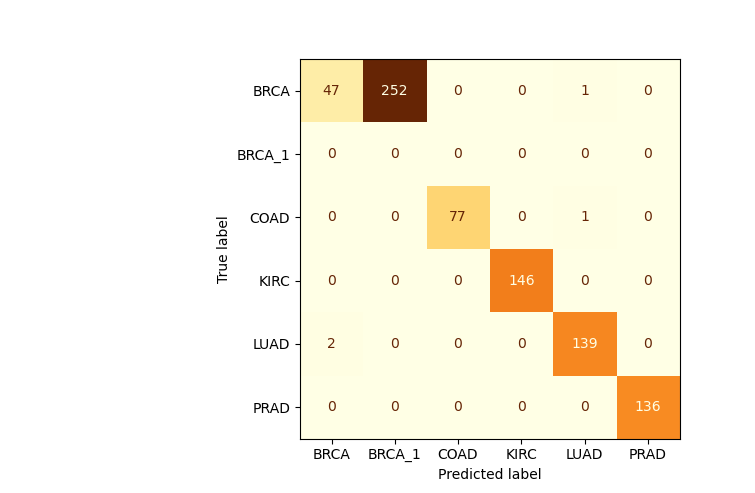
\includegraphics[scale=.45]{CAH/confusion789.png}
	
	Et le taux de mal classé est de 0.499 $\%$ (taux très semblable à celui obtenu à la méthode des K-means)
	
	Et nous pouvons constater de nouveau que c'est la catégorie de Cancer BRCA qui se scinde en 2.\\
	Si nous changeons le seuil et le choisissons à 1500  nous aurons les 5 classes de cancers :\\
	\hspace*{2cm}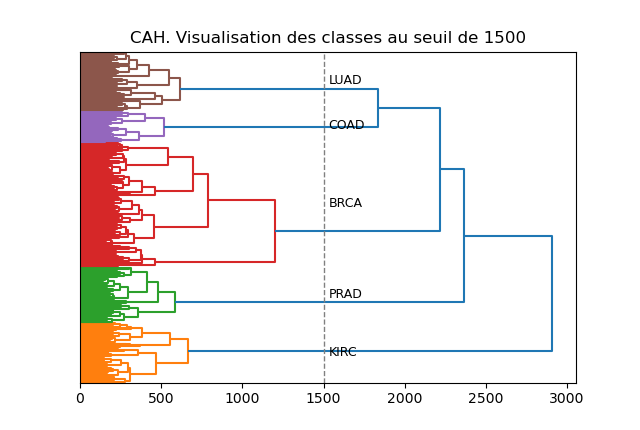
\includegraphics[scale=.5]{CAH/arbre1500.png}\hspace{1.8cm}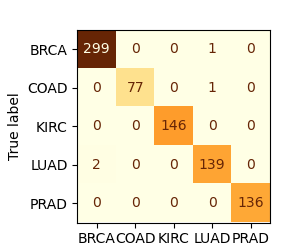
\includegraphics[scale=.8]{CAH/confusion1500.png}
	
	Le taux de mal classé est de : 0.499 $\%$
	
	\section{Analyse discriminante}
	
	Il a été fait le chois d'effectuer une analyse discriminante linéaire et quadratique sur l'ensemble des données et d'effectuer une validation croisée (entraînement sur les 2/3 des données et test sur 1/3 des données, le choix est fait aléatoirement, et ce choix est refait 10 fois puis moyenné).
	
	
	\section{Conclusion}
	
	\begin{enumerate}
		\item \textbf{BRCA :} le phénomène constaté semble pertinent à être considéré, en effet en faisant une rapide recherche nous constatons que le cancer BRCA se scinde en 2 types de cancer. Cette éventuelle interprétation, n'est appuyé que par une simple et courte recherche sur internet, l'appui d'un ou d'une expert aurait été intéressante.
		
		\item Une chose curieuse que je n'ai pu expliquer est que la matrice de variance interclasse (est à priori non inversible) mais cela ne provoque pas d'erreur sur l'analyse discriminante linéaire (contrairement à l'analyse discriminante quadratique) pour l'algorithme fourni par la bibliothèque scikit-learn.
	\end{enumerate}
	
	
	
\end{document}